
\documentclass[11pt]{article}
\usepackage{fullpage,amsmath,amsfonts,mathpazo,microtype,nicefrac}
\usepackage{graphicx}
\graphicspath{{Figures/}} % Specifies the directory where pictures are stored
\usepackage{caption}
\usepackage{subcaption}
\usepackage{listings}
\usepackage{setspace}
\usepackage{multirow}


\title{CS207 Algorithm: K-Means Clustering}
\author{Amy Lee \and Vinay Subbiah \and Victor Lei \and Isadora Nun \and Fanny Heneine}

\begin{document}
\maketitle{}

\pagestyle{plain}
\pagenumbering{arabic}

\section*{Introduction}
K-means is an unsupervised learning algorithms that solves the clustering problem by partitioning and classifying $n$ observations of a given data set into a fixed number $k$ of clusters\footnote{Data Clustering algorithm at https://sites.google.com/site/dataclusteringalgorithms/k-means-clustering-algorithm}.
It defines $k$ centroids, one for each cluster and each observation belongs to the cluster with the nearest mean $\mu_k$. The clusters tend to be of comparable spatial extent and this process results in a partitioning of the data space into Voronoi cells \footnote{A Voronoi diagram is a partitioning of a plane into regions based on distance to points in a specific subset of the plane}. The objective function to be minimized for the algorithm is a squared error function:
\begin{gather}
\sum_{k=1}^{K}\sum_{x_i \in c_k}\Big|\Big|x_i-\mu_k\Big|\Big|^2 \\
\mu_k=\frac{1}{C_k}\sum_{x_i \in c_k} x_i
\end{gather}

\noindent where $\big|\big|x_i-\mu_k\big|\big|$ is the Euclidean distance between $x_i$ and $\mu_k$ (the mean of the $k^{th}$ cluster), $c_k$ is the set of points of the $k^{th}$ cluster and $K$ is the number of clusters. \\


\noindent After the first classification has been done, the $\mu_k$ new centroids are recalculated as the mean of all points belonging to each cluster, and the clustering of observations is re-conducted and updated. The process is iterative until the $k$ centroids do not change location anymore: The algorithm has converged, but the solution might be a local minimum. This is known as Lloyd’s algorithm\footnote{https://datasciencelab.wordpress.com/2013/12/12/clustering-with-k-means-in-python/}


\begin{equation}
C_k=\{x_i: \big|\big|x_i-\mu_k\big|\big| \leq \text{all } \big|\big|x_i-\mu_l\big|\big|\}
\end{equation}

\noindent For the starting set of centroids, several methods can be employed, for instance random assignation.


\section*{Naive Implementation in Python}\
As a first step, we implemented a K-means clustering algorithm using Numpy. The snippets of the code are shown below in figure \ref{naive}.
	
		\begin{figure}[h!]
			\centering 
			\begin{subfigure}{0.7\textwidth}
				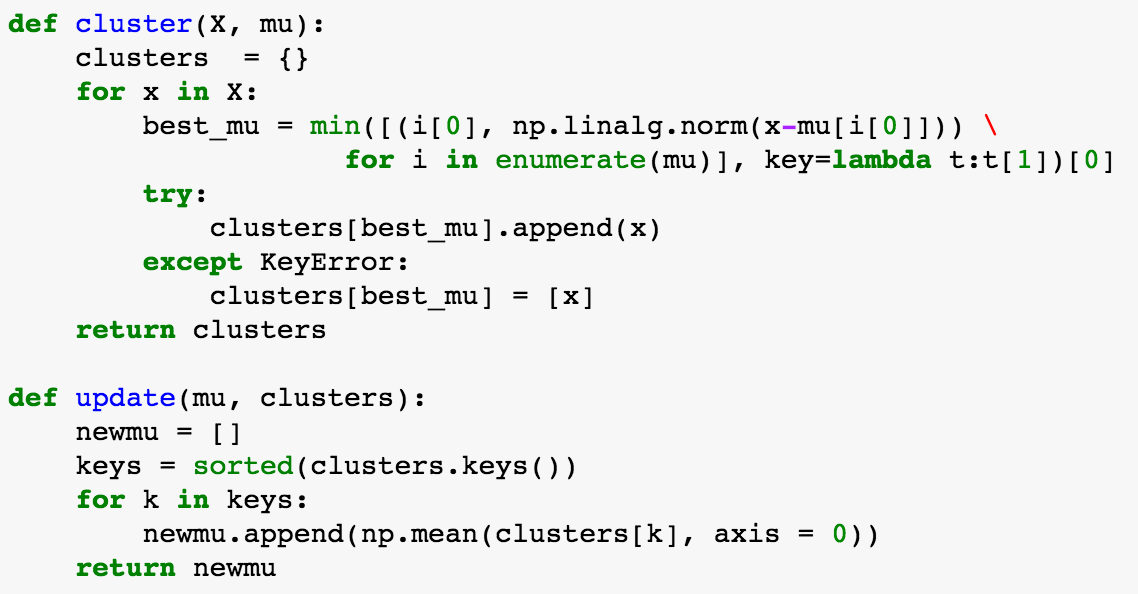
\includegraphics[width=\textwidth]{Figures/Imp1.png}
			\end{subfigure}
			\quad
			\begin{subfigure}{0.7\textwidth}
				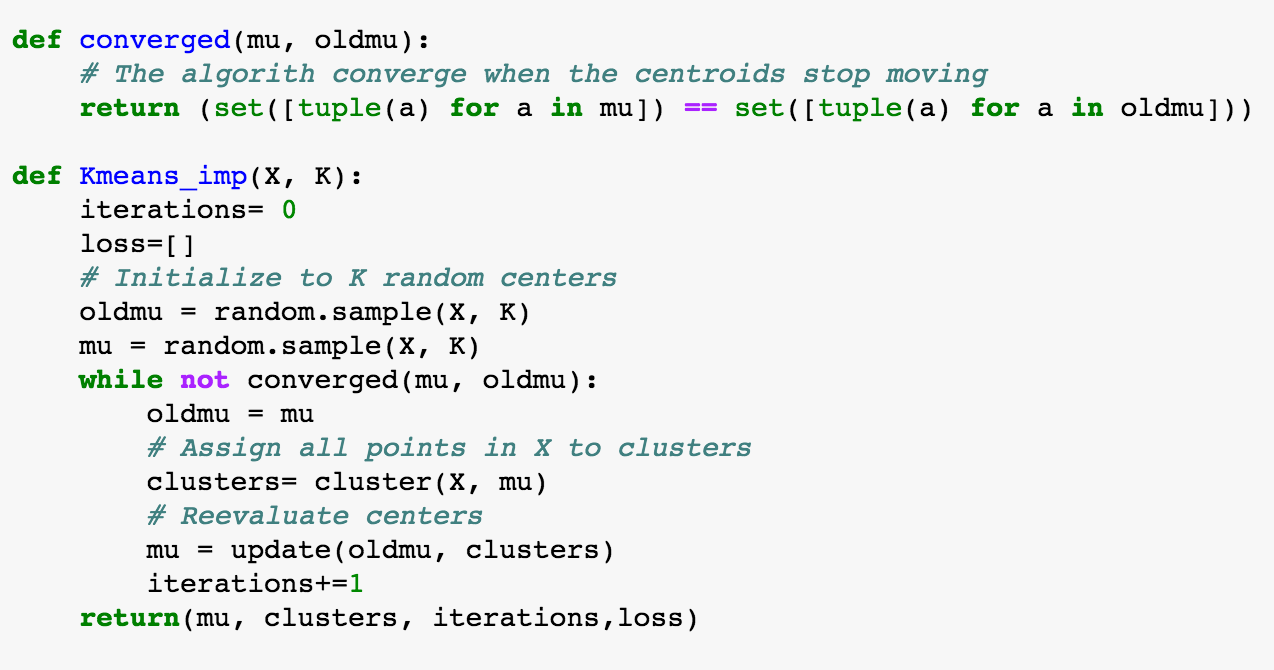
\includegraphics[width=\textwidth]{Figures/Imp2.png}
			\end{subfigure} 
			\caption{Python and Numpy naive implementation}
			\label{naive}
		\end{figure}
\noindent The process starts by randomly sampling the cluster centers. Next, the points are assigned to each cluster using the minimum Euclidean distance and the centers are then re-evaluated. A while loop is used to ensure the process is iterative until the cluster barycenters do not update anymore and remain the same.\\

\noindent To ensure validity of the algorithm, a dataset of size 5000 is generated using the \verb|make_blobs| function, which generates isotropic Gaussian blobs for clustering around centers chosen by the user (in this case three centers at (1, 1), (-1, -1) and (1,-1)). The centroids resulting from the naive implementation match these centers.
The Scikit-Learn results\footnote{Example taken from:http://scikit-learn.org/stable/auto-examples/cluster/plot-mini-batch-kmeans.html}, are plotted in figure \ref{results}. We must note that the sklearn algorithm includes two implementation: The Kmeans and MiniBatch Kmeans, which differences will be discussed later on.

	\begin{figure}[ht!] 
		\centering
		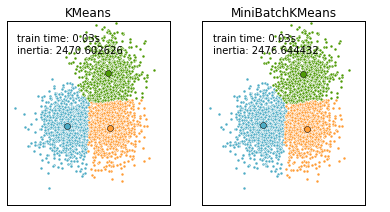
\includegraphics[scale=0.8]{Figures/kmeans.png}
		\caption{Sklearn Implementation Results}
		\label{results}
	\end{figure}

\section*{Comparison}

We compare the performance of our naively implemented algorithm and the Scikit-Learn modules (both KMeans and MiniBatch KMeans) on several generated datasets of increasing size using again the \verb|make_blobs function| function with the same three centers. To ensure consistency in our comparison, we initialize all input similarly: the standard deviation is equal across each clustering, three clusters are generated and the batch size is always 45 for the miniBatch algorithm. A discussion of the best input parameter is  beyond the scope of the paper.  Our naive implementation is inherently slower, and the difference grows exponentially with the size of the dataset,  as illustrated in figure \ref{comp} below. Two figures are shown as the full figure on the left hand side does not clearly illustrate the difference in time for smaller datasets due to its scale.

\begin{figure}[h!]
	\centering 
	\begin{subfigure}{0.48\textwidth}
		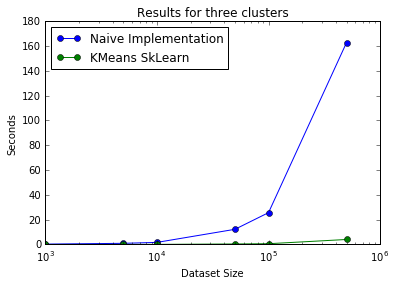
\includegraphics[width=\textwidth]{Figures/Comparison2.png}
		\caption{Small datasets $\leq 10^4$}
	\end{subfigure}
	\quad
	\begin{subfigure}{0.48\textwidth}
		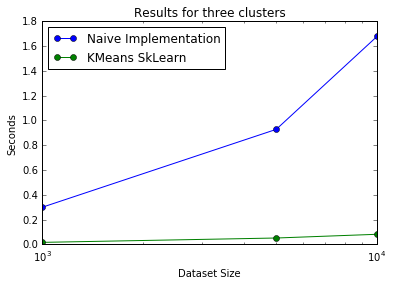
\includegraphics[width=\textwidth]{Figures/Comparison.png}
		\caption{Bigger Datasets  $> 10^4$}
	\end{subfigure} 
	\caption{Comparison between naive implementation and Scikit-Learn K-Means Project}
	\label{comp}
\end{figure}

	

\section*{Optimization}
When comparing both Scikit-Learn Project implementations, which primary module is \verb|k_means_.py|, with our naive Python implementation, an obvious gap in performance is observed. The performance of the SkLearn project algorithms has been drastically more efficient, with a much shorter convergence time.  The naive implementation performance is quite slow, with 160 seconds required to group into three clusters half a million data points. Therefore, the need for optimization becomes obvious in order to handle bigger datasets, but also to decrease the number of iterations required. \\

\noindent In this section, we examine how the algorithm is optimized to improve convergence time. The Scikit-Learn KMeans includes several optimizations components, both within the pure Python implementation and by making use of Cython. In addition, a variant of KMeans (Mini Batch KMeans) is detailed to analyze how its specificities enhances efficiency.  

\subsection*{Pure Python Optimization tools}
The first optimization consists of careful seeding. The algorithm selects initial cluster centers for k-mean clustering in a smart way to speed up convergence, by decreasing the number of iterations needed to reach a solution. \\

\noindent Indeed, we have seen that the algorithm converges but maybe to a local minimum. This is a directly impacted by the initialization of the centroids in the first step, which requires several computation of the algorithm (each one generating different initial centroids) before converging. The Scikit Learn algorithm provides a solution that reduces computation times and speeds up the algorithm by providing a method that solves this issues: The k-means++ initialization generates centroids that are distant from each other, which yields results that are better than when using randomly chosen centroids. This first optimization tool reduces computation time by 25\%: We run the algorithm on the same dataset with and without the input parameter "init='k-means++'", and we see the run time reduce from 0.057 seconds to 0.044 seconds. \\

\noindent Another feature implemented in K-means is pre-computing distance with a preliminary check for memory issues: When pre-computing the distances, the algorithm creates a $m$ by $n$ matrix with $m$ being the number of clusters and $n$ the number of samples. Therefore this feature is activated only under a certain threshold of 12 million entries, to ensure that memory is not eaten up.\\

\noindent Finally, K-means also provides the possibility of parallel computing to optimize running time. By using the $n_{jobs}$ input to K-means (which has a default value of 1), and assigning it a positive value, the algorithm will use the number of assigned processors. This parallelization of k-means runs increases speeds but also increases the memory cost, as several copies of centroids need to be stored. 

\subsection*{Cython}
Cython is an optimising static compiler that creates an interface between Python and C, allowing the combination of higher-level and lower-level code. It allows users to easily write Python code that calls back and forth from C: Cython transforms Python code into a format that compiles into C code\footnote{Cython C-Extension for Python: http://cython.org/}. The main advantage of this extension resides in the fact that the speed of C, which results from the ability to compile, can now be incorporated into Python. Cython therefore allows developers to improve the performance of their code without having to deal with the intricacy of lower-level coding. \\ 

\noindent In the Scikit-Learn \verb|k_means_.py| module, several components are written in Cython: \verb|_k_means.pyx| and \verb|_k_means\_elkan.pyx| are imported and used within the module. \verb|_k_means.pyx| is a Cython code for efficient computation of distances and labels within dense matrices or Compressed Sparse Row Format (or sparse CSR) matrix representation\footnote{Matrix in which most of the elements are zero and which compresses the row indices}. Numpy operations are implemented in C to compute label assignment and inertia\footnote{Sum of squared distances to the centroids} and to calculate cluster means, for either a sparse or dense matrix, as functions exist for both scenarios. It is also used in the Mini batch variant, which we discuss below, to conduct incremental update of the centers and compute squared difference and inertia of the sampled obeservations. This association between C and Numpy allows faster operations.\\

\noindent On the other hand, \verb|_k_means\_elkan.pyx| is a variant of the algorithm beyond the scope of the paper. It is only called either when the data is dense or if the user calls algorithm="elkan" and uses the triangle inequality to speed up k-means for dense data: It calculates an upper and lower bound distance for each sample. 

\subsection*{Mini Batch Kmeans}
The MiniBatchKMeans is a different version of the KMeans algorithm which uses the same function to be minimized but samples subsets of the input data to reduce the computation time. These subsets are called mini-batches, and are randomly sampled in each iteration. The MiniBatchKmeans algorithm steps are as follows: Samples are extracted from the dataset (this is a mini-batch) and are allocated to the closest centroid. The centroids are then updated but withing each sample, leading to incremental updates of their position. As explained in the Scikit Learn documentation\footnote{SKLearn Clustering Documentation: http://scikit-learn.org/stable/modules/clustering.html}:
"For each sample in the mini-batch, the assigned centroid is updated by taking the streaming average of the sample and all previous samples assigned to that centroid". 
This leads to a important decrease in the rate of change for a centroid over time.\\

\noindent This algorithm therefore converges much faster than the standard KMeans as the amount of computation that leads to a local minimum convergence is diminished. The difference in convergence time is negligible for small datasets ($\leq 10^5$), as seen in figure \ref{minibatch} but becomes drastic when the size increases, as seen in figure \ref{minibatch2}.\\

\begin{figure}[t!]
	\centering 
	\begin{subfigure}{0.48\textwidth}
		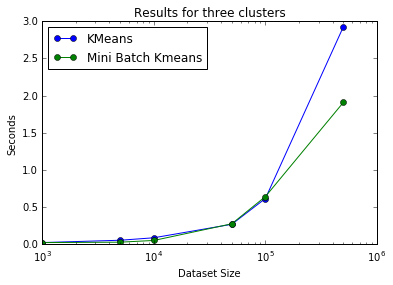
\includegraphics[width=\textwidth]{Figures/minibatch.png}
		\caption{Small datasets $\leq 10^4$}
		\label{minibatch}
	\end{subfigure}
	\quad
	\begin{subfigure}{0.48\textwidth}
		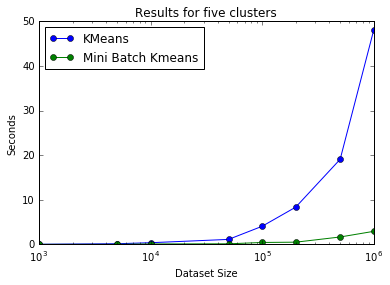
\includegraphics[width=\textwidth]{Figures/minibatch2.png}
		\caption{Bigger Datasets $> 10^4$}
			\label{minibatch2}
	\end{subfigure} 
	\caption{Mini Batch KMeans Agorithm Convergence time}
\end{figure}

\noindent We must however note that convergence time is reduced at a cost: The mini batch KMeans results are slightly worse than the ones generated by KMeans.


\section*{Conclusion}
As a conclusion, different tools are combined to enhance the efficiency of the KMeans  algorithm module, from the implementation of pure Python improvements to the use of Cython to enhance performance. The combination of these tools makes this project a very strong clustering algorithm. However, as performance gets slower for large datasets ($>10^4$), the developers have implemented an even better-performing algorithm (Mini Batch KMeans within the same module) that gives the ability to perform clustering of a datasets of the order $10^6$ in less than 5 seconds, by using random subsets of the data. \\


\end{document}